\usepackage{graphicx}
\usepackage{rotating}
%\setbeamertemplate{caption}[numbered]
\usepackage{hyperref}
\usepackage{caption}
\usepackage[normalem]{ulem}
%\mode<presentation>
\usepackage{wasysym}
\usepackage{amsmath}

\setbeamertemplate{navigation symbols}{}
\institute{Department of Political Science}
\titlegraphic{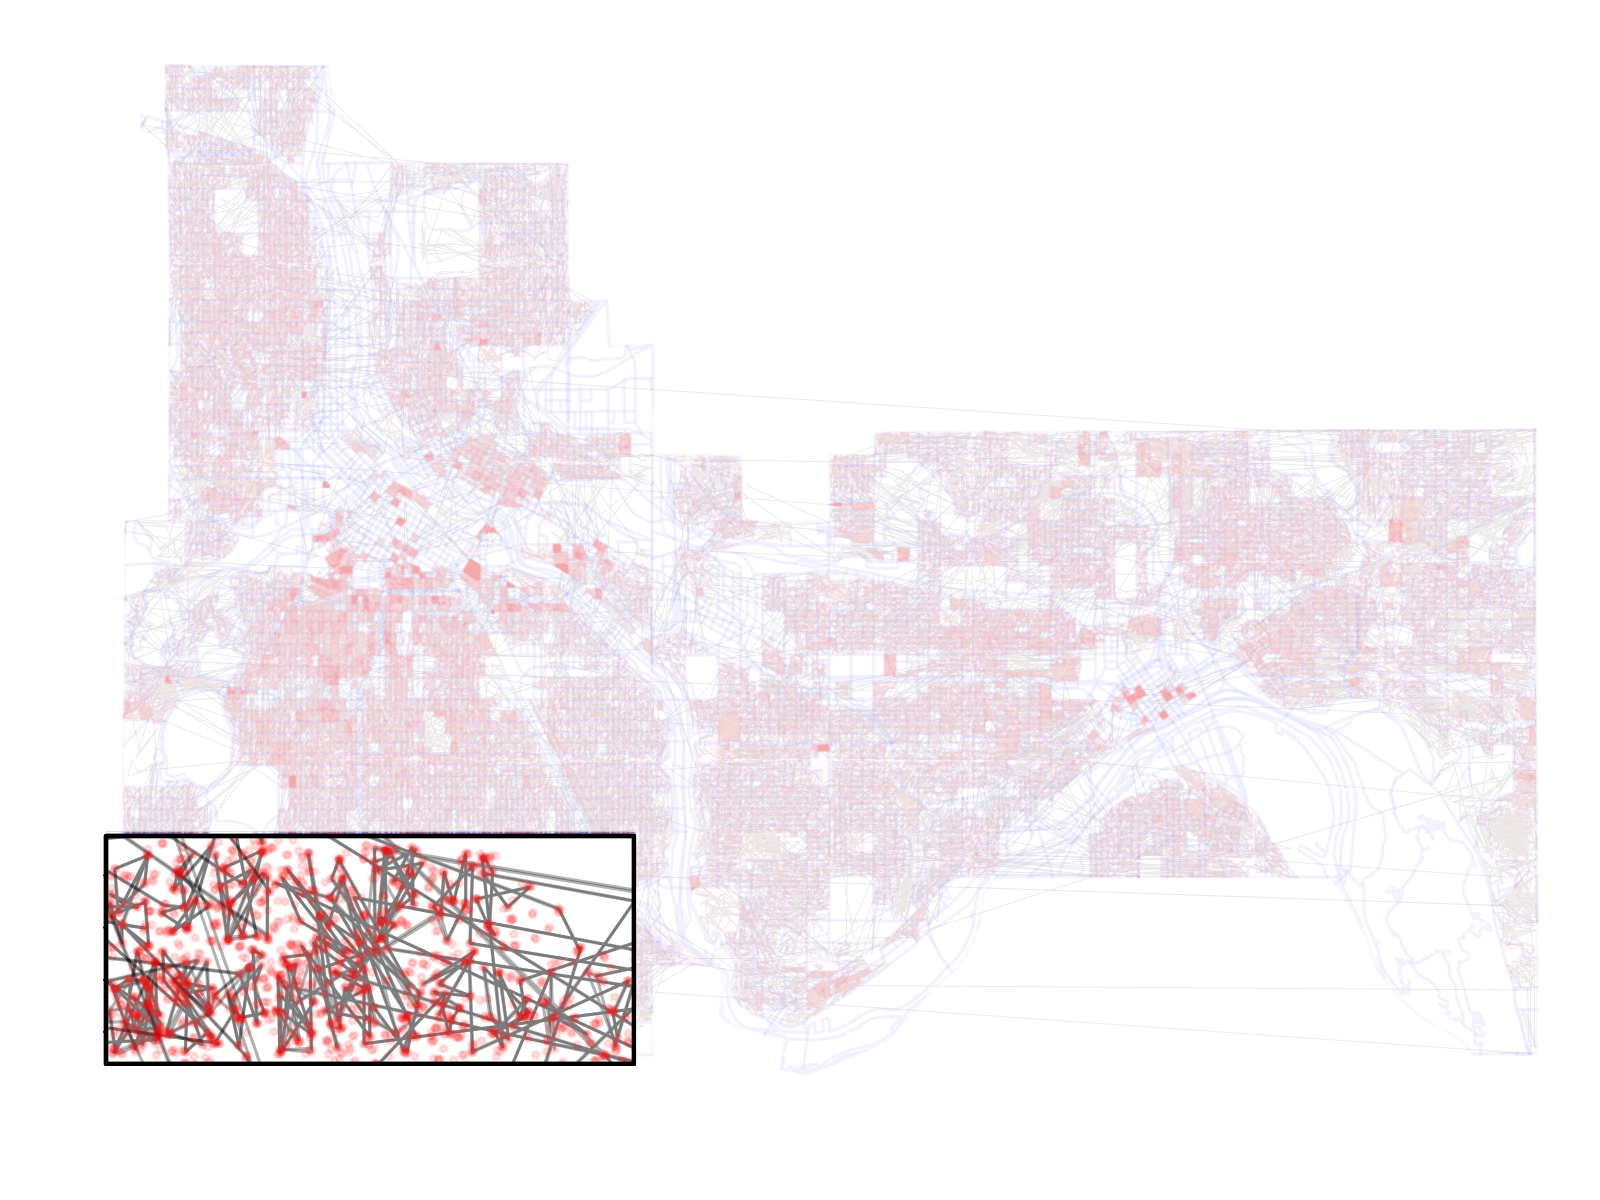
\includegraphics[width=.4\paperwidth]{\string cover/minn.png}}
\setbeamertemplate{title page}[empty]

\setbeamerfont{subtitle}{size=\small}

\setbeamercovered{transparent}

\definecolor{clemsonpurple}{HTML}{522D80}
\definecolor{clemsonorange}{HTML}{F66733}

\setbeamercolor{frametitle}{fg=clemsonpurple,bg=white}
\setbeamercolor{title}{fg=clemsonpurple,bg=white}
\setbeamercolor{local structure}{fg=clemsonpurple}
\setbeamercolor{section in toc}{fg=clemsonpurple,bg=white}
%\setbeamercolor{subsection in toc}{fg=clemsonorange,bg=white}
\setbeamercolor{item projected}{fg=clemsonpurple,bg=white}
\setbeamertemplate{itemize item}{\color{clemsonpurple}$\bullet$}
\setbeamertemplate{itemize subitem}{\color{clemsonpurple}\scriptsize{$\bullet$}}
\let\Tiny=\tiny

\AtBeginPart{}
\AtBeginSection{}
\AtBeginSubsection{}
\AtBeginSubsubsection{}
\setlength{\emergencystretch}{0em}
\setlength{\parskip}{0pt}